% !TEX root = ../foundations.tex

\section{Manifolds with corners}\label{S: manifolds with corners}

In this section, we provide an overview of manifolds with corners, which are the main geometric objects in the definitions of geometric chains and cochains.
Our main references for this material are Joyce \cite{Joy12} and Margalef--Roig and Outerelo Dominguez \cite{MaDo92}. In \cite{MaDo92}, manifolds with corners (which they simply call ``manifolds'') may be infinite-dimensional and may fail to be Hausdorff, so there is some work involved in seeing that their definition agrees with Joyce's when one assumes, as we shall, that all spaces are finite-dimensional, Hausdorff, and second countable.

By \textbf{smooth} we always mean differentiable of all orders.
Throughout the paper, all manifolds and maps will be in the smooth category unless noted otherwise.

\begin{definition}\label{D: smooth}
	If $A \subset \R^n$ and $B \subset \R^m$ are any subsets, we say that $f \colon A \to B$ is \textbf{smooth} if it extends to a smooth map from an open neighborhood of $A$ to $\R^m$.
	We say that $f$ is a \textbf{diffeomorphism} if $f$ is a homeomorphism and both $f$ and $f^{-1}$ are smooth\footnote{Joyce requires $n = m$ in his definition for $f$ to be a diffeomorphism.
	But suppose $f$ is a diffeomorphism as defined here and, without loss of generality, $n>m$.
	Let $\R^m \subset \R^n$ in the usual way.
	Then as $f$ extends to a smooth map from a neighborhood of $A$ to $\R^m$, we can certainly consider $f$ as extending to a smooth map from a neighborhood of $A$ to $\R^n$.
	Similarly, as $f^{-1}$ extends to a smooth map from a neighborhood of $B$ in $\R^m$ to $\R^n$, we can extend $f^{-1}$ to a neighborhood $B$ in $\R^n$ by precomposing with the projection $\R^n \to \R^m$.
	So diffeomorphisms in our sense can be made into diffeomorphisms in Joyce's sense, and obviously vice versa.}.
\end{definition}

With this definition, the notions of smooth charts and atlases for manifolds in the standard setting can be extended to define (smooth) manifolds with corners; see \cite[Section 2]{Joy12}: An $n$-dimensional chart $(U,\phi)$ of the space $W$ has domain $U$ an open subset of $\R^n_k = [0,\infty)^k \times \R^{n-k} \subset \R^n$, and $\phi$ is a homeomorphism from $U$ to $\phi(U) \subset W$.
Two $n$-dimensional charts $(U,\phi)$ and $(V,\psi)$ are compatible if $\psi^{-1}\phi \colon \phi^{-1}(\phi(U) \cap \psi(V)) \to \psi^{-1}(\phi(U) \cap \psi(V))$ is a diffeomorphism of subsets of $\R^n$.
An $n$-dimensional atlas for $W$ is a family of pairwise compatible $n$-dimensional charts that cover $W$, and an $n$-dimensional manifold with corners is a second countable Hausdorff space with a maximal $n$-dimensional atlas.
Our condition that $W$ be second countable is slightly more restrictive than Joyce's definition, which requires only that $W$ be paracompact.

The reason for our additional restriction is that we choose to work entirely with subspaces of $\R^\infty$ in order to have a set of such objects, so rather than directly employ Joyce's definition, we define manifolds with corners for the purposes of this text as follows.

\begin{definition}\label{D: MWC}
	An $n$-dimensional \textbf{manifold with corners} $W$ is a subspace of some $\R^N \subset \R^\infty$ such that each point of $W$ possesses a neighborhood diffeomorphic to an open subset of $\R^n_k$ for some $k$.
\end{definition}

We note that these local diffeomorphisms provide charts $\phi \colon U \subset \R^n_k \to W$, and these charts are compatible, with $\psi^{-1}\phi \colon \phi^{-1}(\phi(U) \cap \psi(V)) \to \psi^{-1}(\phi(U) \cap \psi(V))$ being a diffeomorphism, even using Joyce's more restrictive notion of diffeomorphism.
These charts collectively give an atlas, and every atlas extends to a unique maximal one.
So our manifolds with corners are also manifolds with corners by Joyce's definition.

On the other hand, Joyce notes in \cite[Remark 2.11 (see also Remark 6.3)]{Joy12} that his version of manifolds with corners agrees with that of Margalef--Roig and Outerelo Dominguez \cite{MaDo92} (except that they consider the much more general case of possibly infinite-dimensional manifolds and possibly of differentiable class $p<\infty$).
They show that when their manifolds with corners (which they simply call manifolds) are second countable, Hausdorff, and of the same finite dimension at all points, they have smooth closed embeddings into finite-dimensional Euclidean spaces \cite[Corollary 11.3.10]{MaDo92} (in particular, the embeddings are proper maps \cite[Proposition 3.3.4]{MaDo92}.
Joyce already assumes his manifolds with corners to be paracompact Hausdorff in \cite[Definition 2.1]{Joy12}, so if we add the second countable condition to his definition,\footnote{For us this will not be a terrible restriction, as in this case being second countable is the same as being paracompact with a countable number of components.
Indeed, every regular second countable space is metrizable \cite[Theorem 34.1]{Mu00}, and hence paracompact, and clearly a locally connected second countable space must have a countable number of connected components.
Conversely, each connected component of a paracompact manifold with corners will be closed, paracompact \cite[Theorem 41.2]{Mu00}, and locally compact (via our charts), so it will be $\sigma$-compact \cite[Appendix A.1]{Sp79}.
A $\sigma$-compact space is Lindelof, and this implies that our manifold with corners can be covered by a countable number of charts, each of which is second countable, which implies second countability.
And then a countable union of second countable spaces is second countable.
So the only effect of our second countability condition is to rule out manifolds with corners in Joyce's sense that have uncountably many connected components.}
any one of Joyce's manifolds with corners is diffeomorphic to a manifold with corners in our sense.

As noted in \cite[Remark 2.11]{Joy12}, his definition of manifolds with corners agrees with those of Cerf \cite{Ce61}, Douady \cite{Doua61}, and Margalef--Roig and Outerelo Dominguez \cite{MaDo92}, and they also correspond to Melrose's t-manifolds in \cite{Melrose}.
As an alternative to citing \cite{MaDo92} in the preceding paragraph, we can also observe that Melrose shows in \cite[Proposition 1.14.1]{Melrose} that t-manifolds can be embedded into manifolds without boundary; so, when second countable, these can then be embedded into Euclidean space by the Whitney Embedding Theorem.

By modeling on $\R^n_k$, our category includes manifolds ($k = 0$ in all charts) and manifolds with boundary ($k \leq 1$ in all charts), as well as cubes and simplices, but not the octahedron, for example, as the cone on $[0,1] \times [0,1]$ is not modeled by any $\R^n_k$.

\begin{comment}
	The smooth real-valued functions on a manifold with corners $W$ are those $f$ such that for each chart $\phi \colon U \subset \R^n_k \to W$ the composition $f \circ \phi \colon U \to \R$ is smooth.
\end{comment}

\begin{definition}
	A map $f \colon W \to M$ between manifolds with corners is {(weakly) \bf smooth} if whenever $(U,\phi)$, $(V,\psi)$ are charts for $W$ and $M$ respectively then
	$$\psi^{-1}f \phi \colon (f\phi)^{-1}\psi(V) \to V$$
	is smooth.

	The \textbf{tangent bundle} of a manifold with corners is the space of derivations of the ring of smooth real-valued functions.
	Analogously to smooth manifolds with boundary, if $(U,\phi)$ is a chart of $W$ then $D\phi$ takes the tangent space to $\R^n$ at $x \in U$ isomorphically to the tangent spaces of $W$ at $\phi(x)$.
	In particular, if $W$ is $n$-dimensional and $x \in W$, then the tangent space at $x$, denoted $T_xW$, is isomorphic to $\R^n$.
\end{definition}

\begin{remark}\label{R: weakly smooth}
	In \cite{Joy12}, Joyce reserves the word \textit{smooth} for weakly smooth maps that also satisfy an additional condition concerning how they interact with the boundaries of their codomains.
	When the codomain is a manifold without boundary, which will be our primary situation of interest, the weaker and stronger notions coincide.
	In the few other cases in which we need to consider maps whose codomains have boundary, in particular boundary immersions and projections of pullbacks, the maps will also satisfy Joyce's stronger condition, though we will never need to utilize this explicitly.
	Thus we will feel justified in simply using the word ``smooth'' throughout, referring the reader to \cite[Definition 3.1]{Joy12} for the full definition.
\end{remark}

While the notion of embeddings of manifolds with corners into manifolds with corners is not straightforward (and it is not clear that these notions in \cite{Joy12} and \cite{MaDo92} agree), the following observation concerning embeddings of manifolds with corners into manifolds without boundary is reassuring.
Suppose a manifold with corners $V$ is embedded in a manifold without boundary $M$, meaning, as in the classical sense, that there is a map $f \colon V \to M$ that is a homeomorphism onto its image and such that $Df$ is injective at each point of $V$; see \cite[Definition 3.3.1 and Theorem 3.2.6]{MaDo92}.
Let $x$ be a boundary point of $V$, and let $(U,\phi)$ be a chart for $V$ at $x$ such that $\phi(0)=x$.
Then, by the definition of smooth maps, $f \phi$ extends smoothly to a neighborhood of the origin in $\R^v$.
As $f$ is an embedding, $D(\phi f)_0$ must be injective, so by classical differential topology there is a neighborhood of $0$ in $\R^v$ on which $f\phi$ extends to an embedding with $x$ in the interior \cite[Section 1.3]{GuPo74}.
In other words, the embedding of $V$ can be extended (locally in some neighborhood of $x$) to an embedding of an ordinary manifold without boundary, and the neighborhood of $x$ in $V$ sits inside a Euclidean neighborhood of this embedding as the diffeomorphic image of $\R^v_k$ for some $k$.

\begin{notation}
	Our default notation for manifolds with corners will be capital letters with the corresponding lower case letter denoting the dimension.
	In other words, $\dim(V) = v$, $\dim(W) = w$, $\dim(M) = m$, etc.
	We generally reserve $M$ for a manifold without boundary.
\end{notation}

\subsection{Boundaries}\label{S: boundaries}

We next need to describe boundaries of manifolds with corners.
Again see \cite[Section 2]{Joy12} for further details.

\begin{definition}
	A point $x$ in an $n$-dimensional manifold with corners $W$ has \textbf{depth} $k$ if there is a chart from an open subset of $\R^n_k$ which sends the origin to $x$.
	The set $S^k(W) \subseteq W$ of elements having depth~$k$ is called the \textbf{stratum of depth $k$}.
	By \cite[Proposition 2.4.]{Joy12}, $S^k(W)$ is an $n-k$ manifold without boundary.
\end{definition}

\begin{example}
	If $W$ is a smooth manifold with boundary in the classical sense, then $S^0(W)$ is its interior, $S^1(W)$ is its boundary, and $S^k(W) = \emptyset$ for $k>1$.
	If $S^k(W) = \emptyset$ for all $k>0$, then $W$ is a manifold without boundary.
\end{example}

When $W$ is a general manifold with corners, the boundary is more naturally a space equipped with a map to $W$, rather than a subspace of $W$.
The reason can be seen, for example, in the teardrop space of \cref{F: teardrop}.
The intuitive boundary here would be homeomorphic to the circle but have a corner at the point of the teardrop.
However, this would not be a smooth manifold with corners.
Instead, we consider the boundary to be homeomorphic to the closed interval together with a map taking both endpoints to the vertex of the teardrop.
To explain in more detail, we have the following definitions.

\begin{figure}[h]
	\documentclass[tikz]{standalone}

\begin{document}
	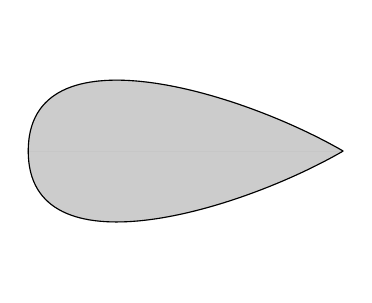
\begin{tikzpicture}[scale=4, rotate=90]
	\coordinate (a) at (0,1.2);
	\coordinate (b) at (0,0.2);

	\draw[out=120, in=180, fill, opacity=.2] (b) to (a);
	\draw[out=120, in=180] (b) to (a);
	\draw[out=60, in=0, fill, opacity=.2] (b) to (a);
	\draw[out=60, in=0] (b) to (a);
	\end{tikzpicture}
\end{document}
	\caption{The 2-dimensional ``teardrop'' is a manifold with corners whose boundary inclusion is not injective.}
	\label{F: teardrop}
\end{figure}

\begin{definition}
	A \textbf{local boundary component} $\beta$ of $W$ at $x \in W$ is a consistent choice of connected component $\mathbf{b}_V$ of $S^1(W) \cap V$ for any neighborhood $V$ of $x$, with consistent meaning that $\mathbf{b}_{V \cap V'} \subset \mathbf{b}_{V} \cap \mathbf{b}_{V'}$.
\end{definition}

Since this notion is local, the number of such components is determined by the depth.
Considering the origin in $\R^n_k$, for any $k \geq 0$, points having depth $k$ have exactly $k$ local boundary components.
As another example, letting $\interval = [0,1]$ and so $\interval^3$ the 3-cube, the set $S^1(\interval^3)$ consists of the interiors of two-dimensional faces, $S^3(\interval^3)$ is the set of eight corners, and any sufficiently small neighborhood of a corner intersects exactly three of the two-dimensional faces.

\begin{definition}\label{D: MWC boundary}
	Let $W$ be a manifold with corners.
	Define its \textbf{boundary} $\bd W$ to be the space of pairs $(x, \bb)$ with $x \in W$ and $\bb$ a local boundary component\footnote{Note that if $x \in S^0(W)$ then $x$ does not have any local boundary components and so does not appear in such a pair.} of $W$ at $x$.
	Define $i_{\bd W} \colon \bd W \to W$ by sending $(x,\bb)$ to $x$.
\end{definition}

In the teardrop example, $i_{\bd W} \colon \bd W \to W$ takes $\interval$ to the topological manifold boundary with both endpoints going to the unique point of $S^2(W)$.
For $\interval^3$, the boundary consists of six closed two-dimensional squares each mapping homeomorphically to a face of the cube.
In general, $|i_{\bd W}^{-1}(x)|$ is equal to the depth of $x$.

As in Douady \cite{Doua61}, $\bd W$ is itself a manifold with corners, and the boundary map $i_{\bd W}$ is a smooth immersion \cite[Theorem 3.4]{Joy12}. Note that $S^1(W)$ will always be diffeomorphic to the interior of $\bd W$, i.e.\ $S^0(\bd W) = S^1(W)$.
Inductively, we let $\bd^k W$ denote $\bd (\bd^{k-1} W)$ with $\bd^0 W = W$, and we let $i_{\bd^k W}$ denote the composite of the boundary maps sending $\bd^k W$ to $W$. The map $i_{\bd^k W}$ takes $S^a(\bd^k W)$ onto $S^{a+k}(W)$, but not, in general, injectively.

\begin{remark}\label{R: bd diff}
	If $f \colon V \to W$ is a diffeomorphism of manifolds with corners then it must, in particular, take components of $S^i(V)$ diffeomorphically onto corresponding components of $S^i(W)$, and, consequently, given a local boundary component $\mathbf{b}$ at a point $x \in V$, the map $f$ picks out a corresponding local boundary component, say $f_*(\mathbf{b})$ in $W$. We obtain a diffeomorphism $f_\bd \colon \bd V \to \bd W$ by $(x,\mathbf{b})\mapsto (f(x),f_*(\mathbf{b}))$ with $fi_{\bd V} = i_{\bd W} f_\bd$.
\end{remark}

If $W$ is a classical smooth manifold with boundary, then we have $\bd^2 W=\emptyset$, but this will not generally be the case for a manifolds with corners.
However, given a map $W \to M$ with either $W$ oriented or the map co-oriented, then $\bd^2 W$ does come equipped with a natural orientation- or co-orientation-reversing $\Z_2$ action.
This will be explained below and is a key component in showing that $\bd$ is suitable for defining boundary maps of geometric chain and cochain complexes.

N.B. When no confusion is likely to occur, we will sometimes abuse notation and use $\bd W$ also to refer to the image $i_{\bd W}(\bd W) \subset W$, which is the boundary of $W$ as a topological manifold in the usual sense.

In the following example, which is a mild generalization of \cite[Example 7.3]{Joy12}, we see $\bd^2 W$ immerse into $W$ in an interesting way.

\begin{example}\label{boundary}
	Consider the quotient $Q$ of $S^n \times \R^2_2$ by the diagonal $\Z_2$ action, where $\Z_2$acts antipodally on $S^n$ and acts by permuting the two coordinates
	of $\R^2_2$.
	The projection of $Q$ onto $S^n / \Z_2 = \R P^n$ defines a fiber bundle with fiber $\R^2_2$.
	Local coordinates can then be used to endow $Q$ with the structure of a manifolds with corners.

	The subspace $S^1(Q)$ is diffeomorphic to $S^n \times (0,\infty)$, and $S^2(Q)$ is diffeomorphic to $\R P^n$.
	The boundary $\bd Q$ is the quotient of $S^n \times \bd \R^2_2$ by $\Z_2$, which is diffeomorphic to
	$S^n \times [0,\infty)$.
	Thus $\bd^2 Q$ is $S^n$, which maps to $S^2(Q)$ by the standard quotient by antipodal action.
\end{example}

In general, Proposition~2.9 of \cite{Joy12} identifies $\bd^k W$ with the set of points $(x,\bb_1,\ldots,\bb_k)$ with $x \in W$ and the $\bb_i$ providing an ordered $k$-tuple of distinct local boundary components of $W$.

\begin{comment}
	% , whose $\bd^3$ is two copies of the symmetric group on three letters.
	% $\bd^1(T \times [0,1])$..., $\bd^2(T \times [0,1])$..., $\bd^3 (T \times [0,1])$...
\end{comment}

Special cases of manifolds with corners, including
manifolds with faces or manifolds with embedded corners \cite{Joy12}, steer clear of the interesting boundary phenomena of \cref{boundary}.
Although, a more restrictive notion should suffice for our application, Lipyanskiy develops geometric cohomology in the current generality, and we appreciate Joyce's careful treatment of transversality in this category, so we use their definitions.

We conclude this section by observing that the product $V \times W$ of two manifolds with corners is naturally a manifold with corners with, by \cite[Proposition 2.12]{Joy12},
$$\bd (V \times W) = (\bd V \times W) \sqcup (V \times \bd W).$$

\subsection{Transversality}

Transversality of smooth maps will play a key role, as this is the condition that assures that intersections or, more generally, pullbacks of manifolds (with corners) are also manifolds (with corners).
Recall that in the classical setting if $f \colon V \to M$ and $g \colon W \to M$ are smooth maps of manifolds without boundary then we say that $f$ and $g$ are \textbf{transverse} if whenever $f(x) = g(y) = z$ for some $x \in V$, $y \in W$, and $z \in M$ we have $Df(T_xV)+Dg(T_yW) = T_z M$.
We here discuss the extension of transversality to manifolds with corners, though only in the case where $M$ is without boundary; as noted in \cite[Remark 6.3]{Joy12}, in this special case Joyce's transversality of manifolds with corners is equivalent to the formulation of transversality in \cite[Section 7.2]{MaDo92}.
More general versions of transversality can be found in \cite[Section 6]{Joy12}.

\begin{definition}{\cite[Special case of Definition 6.1]{Joy12}}
	Let $f \colon V \to M$ and $g \colon W \to M$ be smooth maps of manifolds with corners to a manifold without boundary.
	We say $f$ and $g$ are \textbf{transverse} if whenever $x \in V$ and $y\in W$ with $f(x) = g(y) = z$, if $x\in S^j(V)$ and $y \in S^k(W)$ then $Df|_{S^j(V)}(T_xS^j(V))+Dg|_{S^k(W)}(T_yS^k(W)) = T_zM$.
	In this case, we often abuse notation by saying that $V$ and $W$ are transverse, leaving the maps tacit.
	Note that the empty map $\emptyset \to M$ is transverse to all other maps.
\end{definition}

Note that in our version of the definition, we use maps of the form $f|_{S^j(V)}$, which are classical smooth maps, as the strata $S^j(V)$ are smooth manifolds. Joyce takes a slightly different approach, first noting that if $f:V\to M$ is a smooth map of manifolds with corners then there is an induced map $Df$ ``in the usual way'' \cite[Definition 3.2]{Joy12} and then restricting $Df$ to $T_xS^j(V)\subset T_xV$ (see also \cite[Proposition 2.4]{Joy12}). However, some thinking through the definitions shows that the resulting spaces $D(f|_{S^j(V)})(T_xS^j(V))$ and $Df(T_xS^j(V))$ are identical, both being the derivations that act on functions $h:M\to \R$ by taking the derivatives of $hf$ in the directions tangent to $S^k(V)$. We somewhat prefer our formulation as it expresses transversality entirely in terms of properties of maps of smooth manifolds (without corners).

The following special case of the definition will also sometimes be useful:

\begin{definition}\label{D: regular value}
If $M = \R$ and $g$ is the inclusion of the point $p$ into $\R$, we will say that $p$ is a \textbf{regular value} for $f \colon V \to M$ when $f$ and $g$ are transverse.
\end{definition}

While this definition of transversality is given in terms of the behavior of $f$ and $g$ on the strata $S^j(V)$ and $S^k(W)$, it is sometimes useful to have a reformulation in terms of the boundaries $\bd^j V$ and $\bd^kW$.
This is the content of \cref{L: simple trans} below, for which we need a further definition.

\begin{definition}\label{D: plain transversality}
Let $f \colon V \to M$ and $g \colon W \to M$ be maps from manifolds with corners to a manifold without boundary.
We say that $f$ and $g$ are \textbf{plainly transverse} if whenever $x \in V$ and $y\in W$ with $f(x) = g(y) = z$ we have $Df(T_xV)+Dg(T_yW) = T_z M$. Note that $x$ and $y$ may be boundary points of $V$ and $W$, the maps $Df$ and $Dg$ being those of \cite[Definition 3.2]{Joy12}.
\end{definition}

\begin{comment}
To be explicit in the case that $x \in V-S^0(V)$ or $y \in W-S^0(W)$ with $f(x) = g(y)$, let $(U_x,\phi_x)$ and $(U_y,\phi_y)$ be charts with $\phi_x(0) = x$ and $\phi_y(0) = y$.
By definition of smoothness, there exist neighborhoods $N_x$ and $N_y$ of $0$ in $\R^v$ and $\R^w$, respectively, so that $f\phi_x$ and $g\phi_y$ extend to smooth maps $\psi_x \colon N_x \to M$ and $\psi_y \colon N_y \to M$.
Then $f$ and $g$ are plainly transverse at $x$ and $y$ if $D\psi_x(T_0 \R^v)+D\psi_y(T_0\R^w) = T_{f(x)}M$.
This property is independent of the involved choices as $D\psi_x(T_0 \R^v)$ is the limit of $D\psi_x(T_{a} \R^v)$ for $a$ taken along any smooth path in $U_x$, and this does not depend on the choice of $N_x$ or $\psi_x$, and similarly for $\psi_y$.
\end{comment}

\begin{lemma}\label{L: simple trans}
	Let $f \colon V \to M$ and $g \colon W \to M$ be maps from manifolds with corners to a manifold without boundary.
	Then $f$ and $g$ are transverse if and only if $fi_{\bd^j} \colon \bd^jV \to M$ and $gi_{\bd^k} \colon \bd^kW \to M$ are plainly transverse for all $j,k$.
\end{lemma}

Note that, a priori, the latter is a stronger condition as it imposes conditions not just on the interior of strata but on their closures.

\begin{proof}
	First suppose $fi_{\bd^j}$ and $gi_{\bd^k}$ are plainly transverse for all $j,k$.
	Suppose $x \in S^j(V)$ and $y \in S^k(W)$ for some fixed $j,k$ and $f(x) = g(y)$.
	The preimage of $x$ under $i_{\bd^j}$ consists of $j!$ points in $S^0(\bd^jV)$, and $i_{\bd^j}$ maps a neighborhood of each such preimage point diffeomorphically to a neighborhood of $x$ in $S^j(V)$, and similarly for $y$.
	Let $\psi_x$ be the inverse diffeomorphism from a neighborhood of $x$ in $S^j(V)$ to a neighborhood of one of the preimages.
	Then $f|_{S^j(V)} = fi_{\bd^j}\psi_x$ in a neighborhood of $x$, and similarly for $y$.
	Since $fi_{\bd^j}$ and $gi_{\bd^k}$ are plainly transverse, and $\psi_x$ and $\psi_y$ are diffeomorphisms, it follows that $f|_{S^j(V)}$ and $g|_{S^k(W)}$ are transverse at $f(x) = g(y)$.

	Conversely, suppose $f|_{S^j(V)}$ and $g|_{S^k(W)}$ are transverse for all $j,k$, and suppose $x \in \bd^jV$ and $y \in \bd^kW$ for some fixed $j,k$ with $fi_{\bd^j}(x) = gi_{\bd^k}(y) = z$.
	Furthermore, suppose $i_{\bd^j}(x) \in S^a(V)$ and $i_{\bd^k}(y) \in S^b(W)$, which implies $x \in S^{a-j}(\bd^j V)$.
	By focusing on local charts, there is a neighborhood of $x$ in $\bd^j(V)$ whose intersection with $S^{a-j}(\bd^j V)$ maps diffeomorphically via $i_{\bd^j}$ onto a neighborhood of $i_{\bd^j}(x)$ in $S^a(V)$, and analogously for $y$.
	Thus, $f|_{S^a(V)}i_{\bd^j}|_{S^{a-j}(\bd^j V)}$ and the analogous $g|_{S^b(W)}i_{\bd^k}|_{S^{b-k}(\bd^k W)}$ are transverse at $f(x) = g(y)$ as they precompose transverse maps with local diffeomorphisms.
	But the image of $D_x(fi_{\bd^j})$ contains the image of $D_x(f|_{S^j(V)}i_{\bd^j}|_{S^{a-j}(\bd^j V)})$ and similarly for $y$, and thus the images of $D_x(fi_{\bd^j})$ and $D_y(gi_{\bd^k})$ must also span $T_{z}M$.
	Therefore, $fi_{\bd^j}$ and $gi_{\bd^k}$ are plainly transverse at $f(x)$.
\end{proof}

\subsubsection{Achieving transversality}

Throughout this text, we will need a series of increasingly more general results guaranteeing that we can make certain maps transverse to each other.
We begin here with two relatively simple cases that will be used in \cref{S: basic properties} to show that geometric cohomology is contravariantly functorial with respect to continuous maps of manifolds without boundary.
We put these first transversality results here, as some of the fundamental ideas will be used in a number of places throughout the text.

Our transversality theorems will be built primarily using some basic tools that can be found in \cite[Section 2.3]{GuPo74}.
In particular, we record the following results, referring the reader to \cite[Section 2.3]{GuPo74} for the proofs\footnote{We rephrase the statements of these theorems slightly to better fit our context and notation.}:

\begin{theorem}[Transversality Theorem]\label{T: GP transversality}
	Suppose $F \colon X \times S \to Y$ is a smooth map of manifolds, where only $X$ has boundary, and let $Z$ be any boundaryless submanifold of $Y$.
	If both $F$ and $F|_{\bd X \times S}$ are transverse to $Z$, then for almost every $s \in S$, both $F(-,s) \colon X \to Y$ and $F(-,s)|_{\bd X} \colon \bd X \to Y$ are transverse to $Z$.
\end{theorem}

\begin{theorem}[$\epsilon$-Neighborhood Theorem]\label{T: epsilon neighborhood}
	For a compact boundaryless manifold $Y$ in $\R^M$ and a positive number $\epsilon$, let $Y_\epsilon$ be the open set of points in $\R^M$ with distance less than $\epsilon$ from $Y$.
	If $\epsilon$ is sufficiently small, then each point $w \in Y_\epsilon$ possesses a unique closest point in $Y$, denoted $\pi(w)$.
	Moreover, the map $\pi \colon Y_\epsilon \to Y$ is a submersion.
	When $Y$ is not compact, there still exists a submersion $\pi \colon Y_\epsilon \to Y$ that is the identity on $Y$, but now $\epsilon$ must be allowed to be a smooth positive function on $Y$, and $Y_\epsilon$ is defined as $\{w \in \R^m \mid |w-y|<\epsilon(y) \text{\ for some\ } y \in Y\}$.
\end{theorem}

These theorems are used in \cite{GuPo74} to prove the following basic transversality result:

\begin{theorem}[Transversality Homotopy Theorem]
	Let $X$ be a smooth manifold with boundary.
	For any smooth map $f \colon X \to Y$ and any boundaryless submanifold $Z$ of the boundaryless manifold $Y$, there exists a smooth map $g \colon X \to Y$ homotopic to $f$ such that $g$ is transverse to $Z$ and $g|_{\bd X}$ is transverse to $Z$.
\end{theorem}

Among other generalizations as we progress, we will extend these results to maps that go from manifolds with corners to manifolds without boundary.
We will also often require that the homotopies take a special form, i.e.\ that they are \textit{universal} homotopies as defined in \cref{D: universal homotopy}.
See, for example, \cref{P: perturb transverse to map}.

When working with transversality, it is often much easier to work with the case where one of the maps is an embedding.
The following technical results will facilitate that and help us to extend the results of \cite{GuPo74} from transversality with respect to submanifolds to transversality with respect to maps.

\begin{lemma}\label{L: proper product}
	Let $f \colon X \to Y$ be an arbitrary map and $g \colon X \to Z$ a proper map.
	Then the map $(f,g) \colon X \to Y \times Z$ given by $(f,g)(x)=(f(x),g(x))$ is proper.
\end{lemma}

\begin{proof}
	Let $K \subset Y \times Z$ be compact.
	Let $\pi_Y,\pi_Z$ be the projections of $Y \times Z$ to $Y$ and $Z$. Then
	\begin{align*}
		(f,g)^{-1}(K) &= \{x \in X \mid (f(x),g(x)) \in K \}\\
		&\subset \{ x \in X \mid g(x) \in \pi_Y(K)\}\\
		&= g^{-1}(\pi_Y(K)).
	\end{align*}
	As $K$ is compact and $g$ is proper, $g^{-1}(\pi_Y(K))$ is compact.
	So $(f,g)^{-1}(K)$ is a closed subset of a compact set, and so compact.
\end{proof}

\begin{corollary}\label{C: embed V}
Let $g \colon W \to M$ be a map from a manifold with corners to a manifold without boundary.
Then for some $k$ there exists a closed embedding $e \colon W \to M \times \R^k$ such that, if $\pi \colon M \times \R^k \to M$ is the projection, then $\pi e = g$.
\end{corollary}

\begin{proof}
	By \cite[Corollary 11.3.10]{MaDo92}, there is a closed embedding $\alpha \colon W \to \R^k$ for some $k$.
	The map $\alpha$ is proper, as if $K$ is a compact subset of $\R^k$, the inverse image $\alpha^{-1}(K)$ is homeomorphic to the intersection of $K$ with the closed set $\alpha(W)$.
	So, by \cref{L: proper product}, the map $(g,\alpha) \colon W \to M \times \R^k$ is proper.
	Further, $\alpha$ is an immersion, so is $(g,\alpha)$.
	In fact, by \cite[Theorem 3.2.6]{MaDo92} and the fact that $M$ and $\R^k$ do not have boundary, a map is an immersion in this context if and only if it is injective on tangent spaces.
	If $\pi_{\R^k} \colon M \times \R^k \to \R^k$ is the projection, the map $\pi_{\R^k}(g,\alpha)$ equals the embedding $\alpha$, so $D(g,\alpha)$ must be injective at each point.
	Similarly, the map $(g,\alpha)$ is itself injective because $\alpha$ is injective.
	So $(g,\alpha)$ is an injective proper immersion, and just as for ordinary manifolds, an injective proper immersion is a closed embedding \cite[Proposition 3.3.4]{MaDo92}.
	Finally, it is clear from the construction that $\pi (g,\alpha) = g$.
\end{proof}

\begin{lemma}\label{L: all transversality is wrt embeddings}
	Let $f \colon V \to M$ and $g \colon W \to M$ be smooth maps from manifolds with corners to a manifold without boundary.
	Let $e \colon W \to M \times \R^n$ be an embedding such that $\pi e = g$, where $\pi$ is the projection $M \times \R^n \to M$.
	Then $f$ and $g$ are transverse if and only if $e$ is transverse to $f \times \id_{\R^n} \colon V \times \R^n \to M \times \R^n$.
\end{lemma}

\begin{proof}
	It suffices to assume that $V$ and $W$ are without boundary.
	Otherwise we can apply the following argument to each pair of strata of $V$ and $W$.

	Suppose that $f$ and $g$ are transverse, i.e.\ that if $f(v) = g(w)$ then $Df(T_vV)+Dg(T_wW) = T_{f(v)}M$.
	For each $w \in W$, we can write $e(w) = (g(w),e_\R(w)) \in M \times \R^n$.
	Now suppose $w \in W$ and $(v,z) \in V \times \R^n$ such that $e(w) = (f \times \id_{\R^n})(v,z)$.
	Then we have $(g(w),e_\R(w)) = (f(v),z)$.
	The image of the derivative of $f \times \id_{\R^n}$ at such a point will span $Df(T_vV) \oplus T_z(\R^{n}) = Df(T_vV) \oplus \R^{n}$, while the derivative of $e$ will take $a \in T_w(W)$ to $Dg(a)+ De_{\R}(a)$.
	But the image of $D(f \times \id_{\R^n})$ already includes $0 \oplus \R^{n}$, so subtracting off the second summand, $D(f \times \id_{\R^{n}})(T_{(v,z)}(V \times \R^n))+De(T_wW)$ contains $Dg(a)$.
	It follows that $D(f \times \id_{\R^{n}})(T_{(v,z)}(V \times \R^n))+De(T_wW)$ contains $Df(T_vV) \oplus 0$, $Dg(T_wW) \oplus 0$, and $0 \oplus \R^n$.
	Since $f$ and $g$ are transverse and $D(f \times \id_{\R^{n}})(T_{(v,z)}(V \times \R^n))+De(T_wW)$ is a vector space, it therefore contains all of $T_{f(v)}M \oplus \R^n = T_{e(w)}(M \oplus \R^n)$.
	So $f \times \id_{\R^n}$ and $e$ are transverse.

	Next suppose $f \times \id_{\R^n}$ and $e$ are transverse and that $f(v) = g(w) \in M$.
	Suppose $e(w) = (g(w),z)$.
	Then $e(w) = (f \times \id_{\R^n})(v,z)$.
	So, by definition and assumption,
	\begin{equation}\label{E: Quillen transverse}
		D(f \times \id_{\R^{n}})(T_{(v,z)}(V \times \R^n))+De(T_wW) = T_{e(w)}(M \times \R^n) = T_{f(v)}M \oplus \R^n.
	\end{equation}
	As $\pi$ is a submersion, the image of this tangent space under $D\pi$ is all of $T_{f(v)}M$.
	But $(D\pi)(De) = D(\pi e) = Dg$, so $(D\pi \circ De)(T_wW) = Dg(T_wW)$.
	Furthermore, letting $\pi_V \colon V \times \R^n \to V$ be the projection, we have $(D\pi)(D(f \times \id_{\R^{n}})) = D(\pi(f \times \id_{\R^{n}})) = D(f\pi_V) = (Df)(D\pi_V)$, so, as $D\pi_V \colon T_{(v,z)}(V \times \R^n) \to T_vV$ is surjective, we have $(D\pi)(D(f \times \id_{\R^{n}}))(T_{(v,z)}(V \times \R^n)) = Df(T_vV)$.
	So applying $D\pi$ to equation \eqref{E: Quillen transverse}, we get $Df(T_vV)+Dg(T_wW) = T_{f(v)}M$, and $f$ is transverse to $g$.
\end{proof}

We now need one more particular technical result that will allow us to achieve transversality while keeping proper maps proper.

\begin{lemma}\label{L: nearby proper homotopy}
	Let $X$ be a topological space and $M$ a manifold without boundary possessing a metric $d$.
	Suppose $f \colon X \to M$ is a proper map.
	Then there exists a function $\varepsilon \colon X \to (0,\infty)$ such that if $g \colon X \to M$ satisfies $d(f(x),g(x)) < \varepsilon(x)$ for all $x \in X$, then $g$ is proper and homotopic to $f$ by a proper homotopy.
	Furthermore, if $X$ is a manifold with corners and $f$ and $g$ are smooth and homotopic by a proper homotopy, then they are homotopic by a smooth proper homotopy.
\end{lemma}

\begin{proof}
	Let $C(X,M)$ be the set of continuous maps from $X$ to $M$.
	By \cite[Proposition 9.2.28]{MaDo92}, there is an open neighborhood $V^f$ of $f$ in the topology $T_s$ on $C(X,M)$ (defined in \cite[Proposition 9.2.1]{MaDo92}) such that every $g \in V^f$ is proper and homotopic to $f$ by a proper homotopy.
	Furthermore, by \cite[Proposition 9.3.9]{MaDo92} there is a local basis at $f$ in the $T_s$ topology consisting of the sets
	$$B_\varepsilon^d = \{g \in C(X,M) \mid d(f(x),g(x)) < \varepsilon (x) \text{ for all } x \in X\}$$
	as $\varepsilon$ ranges over all continuous functions $X \to (0,\infty)$.
	So, in particular, there is an $\varepsilon$ such that $B_\varepsilon^d \subset V^f$, which proves the first part of the lemma.
	When $X$ is a manifold with corners and $f$ and $g$ are smooth, we can take the proper homotopy between them to be proper and smooth by \cite[Proposition 9.2.35]{MaDo92}; note that $X$ satisfies the hypotheses of having partitions of unity by \cite[Corollary 1.5.14]{MaDo92}.
\end{proof}


We now apply the above results to demonstrate two transversality theorems that we will need in \cref{S: cohomology pullback} to obtain contravariant functoriality of geometric homology and cohomology.
We will see various alternative, and in some cases fancier, versions of these theorems below.
See, for example, \cref{P: ball stability,P: perturb transverse to map}.

\begin{theorem}\label{T: basic trans}
	Let $f \colon M \to N$ be a continuous map of manifolds without boundary, and let $g \colon V \to N$ be a smooth map from a manifold with corners.
	Then there is a homotopy $h \colon M \times I \to N$ such that $h(-,0) = f$, and $h(-,1)$ is smooth and transverse to $g$.
	Furthermore, if $f$ is proper, then there is such an $h$ so that both $h$ and $h(-,1)$ are proper.
\end{theorem}
\greg{Old version of this had a bit about $M$ having boundary and keeping the $f$ restricted to boundary fixed if it was already good. Got rid of that to add proper without trouble. Need to make sure I never really need the boundary thing. Changeover around 9-11-23. Though see also the next theorem I added for homotopies.}

\begin{proof}
	By \cref{C: embed V}, there is a closed embedding $e \colon V \to N \times \R^k$ that satisfies the hypotheses of \cref{L: all transversality is wrt embeddings}, so by that lemma it suffices to find a homotopy such that $h(-,0) = f$ and $h(-,1) \times \id_{\R^k} \colon M \times \R^k \to N \times \R^k$ is smooth and transverse to $e(V)$.

	We first find a homotopy from $f$ to a smooth map.
	This can be done by the smooth approximation theorem; see \cite[Corollary 9.2.31]{MaDo92}.
	Furthermore, if $f$ is proper, then we can take the smooth map and the homotopy between it and $f$ to be proper by \cite[Corollary 9.2.36]{MaDo92}.
	So we assume for the rest of the proof that this first homotopy has been completed and that $f$ is a smooth map.
	\begin{comment}
	We will next construct our homotopy to achieve transversality without consideration of whether or not $f$ is already transverse to $g$ on $\bd M$, and then we show how to modify the construction for that case.
	\end{comment}

	Next, we can think of $N$ as properly embedded in some $\R^K$ by the Whitney Embedding Theorem \cite[Section 1.8]{GuPo74}, and we give $N$ the corresponding metric.
	We let $N_\epsilon$ be an $\epsilon$ neighborhood of $N$ in $\R^K$ with submersion $\pi \colon N_\epsilon \to N$ (see \cref{T: epsilon neighborhood}).
	Let $D$ be the open unit ball in $\R^K$.
	We define a smooth composite map $H \colon M \times D \to \R^K \to N$ by
	$$H(x,s) = \pi(f(x)+ \eta(x)s)$$
	where $\eta \colon M \to (0,\infty)$ is defined as follows.

	First, so that $H(x,s)$ will be well defined, we want $f(x)+ \eta(x)s$ to land in $N_\epsilon$ for all $x$, and for this it is sufficient to have $0< \eta(x) < \epsilon(f(x))$.
	If $f$ is not proper or we do not need the last clause of the theorem to hold, any such $\eta$ will be sufficient.
	If $f$ is proper and we want the last clause of the theorem to hold, then we next choose a function $\varepsilon \colon M \to (0,\infty)$ to meet the requirements of \cref{L: nearby proper homotopy} with $d$ being the distance on $N$ chosen above.
	Letting $|\cdot|$ be the norm on $\R^K$, we then want to choose $\eta$ so that $|f(x) - H(x,1)| < \varepsilon(x)$.
	Clearly, $|f(x) - (f(x)+ \eta(x)s)| = |\eta(x)s| < \eta(x)$, and by definition $\pi$ takes points of $N_\epsilon$ to the nearest point in $N$. So, assuming $f(x)+ \eta(x)s \in N_\epsilon$, then $|f(x)+ \eta(x)s - \pi(f(x)+ \eta(x)s)| < \eta(x)$, as $f(x) \in N$.
	So by the triangle inequality, $|f(x) - H(x,s)| < 2\eta(x)$.
	Thus if we take $\eta(x) < \min(\epsilon(f(x)), \varepsilon(x)/2)$, we will have $H$ well defined and $|f(x) - H(x,s)| < \varepsilon(x)$ for any $x \in M$ and $s \in D$ by \cref{L: nearby proper homotopy}.

	Now, we have $H(x,0) = \pi(f(x)) = f(x)$, and, since $\eta(x)>0$ for all $x$, the map $(x,s) \to f(x)+ \eta(x)s$ is a submersion onto its image in $\R^K$; in fact, for $x$ fixed, $H(x,s)$ maps $D$ linear onto a ball neighborhood of $f(x)$.
	As $\pi$ is also a submersion, so is $H$, and then $H \times \id_{\R^k} \colon M \times D \times \R^k \to N \times \R^k$ is a submersion.
	In particular, $H \times \id_{\R^k}$ is transverse to $e(V)$ and to $e(S^i(V))$ for each stratum $S^i(V)$ of $V$.
	We can now apply the Transversality Theorem, (\cref{T: GP transversality}, though with the parameter space $D$ in a slightly nontraditional location in the ordering of factors) to obtain that $H(-,s) \times \id_{\R^k}$ is transverse to $e(V) \times \R^k$ for almost every $s \in D$ and similarly for each $S^i(V)$.
	Since $V$ has a finite number of strata, and since the intersection of a finite number of sets whose complements have measure zero is another set whose complement has measure zero, it holds for almost every $s \in D$ that $H(-,s) \times \id_{\R^k}$ is transverse to every stratum of $V$.
	Now let $s_0$ be one such $s$, and let $h \colon M \times I \to N$ be given by $h(x,t) = H(x,ts_0)$.
	Then $h(x,0) = H(x,0) = \pi(f(x)) = f(x)$, and $h(-,1) = H(-,s_0)$ is smooth and transverse to every stratum of $V$ by \cref{L: all transversality is wrt embeddings}.
	Furthermore, if $f$ is proper, then by \cref{L: nearby proper homotopy} and our choice of $\eta$, the map $h(-,1)$ is proper and if necessary we can replace $h$ with a proper homotopy from $f$ to $h(-,1)$. \qedhere

	\begin{comment}
	If $f|_{\bd M}$ is already transverse to $g$, we modify the construction as follows: Let $\rho \colon M \to [0,1]$ be a smooth function that is $0$ on $\bd M$ and $>0$ on $M-\bd M$.
	Then we define
	$$H(x,s) = \pi(f(x)+ \epsilon(f(x))\rho(x)s).$$
	Then when $x \in \bd M$, we have $H(x,s) = \pi(f(x)) = f(x)$, so $h$ is constant along $\bd M$.
	For $x \notin \bd M$, the argument goes through exactly as above.
	\end{comment}
\end{proof}

Our second theorem will be applied below when $M$ is of the form $Y \times I$ for $Y$ a manifold without boundary in order to improve a homotopy between maps that are both transverse to another given map $g$ to a homotopy that is transverse to $g$.

\begin{theorem}\label{T: homotopy trans}
	Let $f \colon M \to N$ be a smooth map from a manifold with boundary to a manifold without boundary, and let $g \colon V \to N$ be a smooth map from a manifold with corners.
	Suppose $\bd f \colon \bd M \to N$ is transverse to $g$.
	Then there is a smooth homotopy $h \colon M \times I \to N$ such that $h(-,0) = f$, $h(-,1)$ is smooth and transverse to $g$, and $h$ fixes $\bd M$, i.e.\ $h(x,t)=f(x)$ for all $x \in \bd M$ and all $t \in I$.
	Furthermore, if $f$ is proper, then there is such an $h$ so that both $h$ and $h(-,1)$ are proper.
\end{theorem}

\begin{proof}
	We continue with the same notation as in the proof of \cref{T: basic trans}.
	In particular, we again assume a closed embedding $e \colon V \to N \times \R^k$ that satisfies the hypotheses of \cref{L: all transversality is wrt embeddings}, a proper embedding of $N$ in $\R^K$ with an $\epsilon$ neighborhood $N_\epsilon$, a submersion $\pi \colon N_\epsilon \to N$, and, in the proper case, a function $\varepsilon \colon M \to (0,\infty)$ to meet the requirements of \cref{L: nearby proper homotopy}.

	In this case $f$ is already assumed to be smooth, but we alter our definition of the map $H \colon M \times D \to \R^K \to N$ as follows.
	Let $\rho \colon M \to [0,1]$ be a smooth function that is $0$ on $\bd M$ and $>0$ on $M-\bd M$ \cite[Proposition 5.43]{Lee13}.
	Then we define
	$$H(x,s) = \pi(f(x)+ \rho(x)\eta(x)s),$$
	where $\eta$ is defined as above.
	Then when $x \in \bd M$, we have $H(x,s) = \pi(f(x)) = f(x)$, so $H$ does not depend on $s$ when $x \in \bd M$.
	The remainder of the argument is now identical to the rest of the proof of \cref{T: basic trans}.
	In particular, for almost all $s$, the restriction of $H(-,s)$ to $M - \bd M$ will be transverse to $g$, while the restriction of $H(-,s)$ to $\bd M$ is just $f(x)$ and so transverse to $g$ by assumption.
	We then define $h$ from $H$ exactly as in the proof of \cref{T: basic trans}, and the conditions in the proper case are satisfied as $\rho(x)\leq 1$.
\end{proof}

\subsection{Pullbacks and fiber products}

When two embedded submanifolds of a manifold meet transversely, their intersection is again a submanifold.
More generally, if two smooth maps of manifolds are transverse, we can form their pullback, also called their fiber product, which is again a manifold.
This construction extends to manifolds with corners mapping into a manifold without boundary.

\begin{definition}\label{D: top pullback}
	Let $f \colon V \to M$ and $g \colon W \to M$ be transverse smooth maps from manifolds with corners to a manifold without boundary.
	Define the \textbf{pullback} or \textbf{fiber product} $V \times_M W$ by
	$$V \times_M W = \{(x, y) \in V \times W \mid f(x) = g(y)\}.$$

	There are canonical maps from $V \times_M W$ to $V$, $W$, and $M$ that respectively take $(x,y)$ to $x$, $y$, and $f(x) = g(y)$.
	\[
	\begin{tikzcd}
		V \times_M W \arrow[r, "g^*"] \arrow[d, "f^*"] & V \arrow[d, "f"] \\
		W \arrow[r, "g"] & M.
	\end{tikzcd}
	\]
	We typically suppress the maps from the notation, though we sometimes label them as in the diagram and sometimes write $f \times_M g \colon V \times_M W \to M$ for the composition around the square.
	We also sometimes write $f^*$ as $\pi_W$ and $g^*$ as $\pi_V$, as these maps are induced by restricting to $V \times_MW$ the projections from $V \times W$ to $V$ and $W$.
	We also often abbreviate $V \times_M W$ as $P$.

	We will generally use the term \textit{pullback} when we want to emphasize $V \times_M W$ with its map to $V$ or $W$, while the \textit{fiber product} is to be considered as mapping to $M$.
	When treating $V \times_M W$ as a pullback, we also sometimes use the notation $g^*V \to W$ or $f^*W \to V$; this notation is consistent with the analogous notation for pullbacks of fiber bundles, which is a special case.
\end{definition}

The reason for the transversality requirement in \cref{D: top pullback} is that this ensures that $V \times_M W$ is itself a manifold with corners, as follows from \cite[Theorem 7.2.7]{MaDo92} or \cite[Theorem 6.4]{Joy12}. In fact, we have the following.

\begin{theorem}\label{pullback}
	Let $f \colon V \to M$ and $g \colon W \to M$ be transverse smooth maps from manifolds with corners to a manifold without boundary.
	Then $V \times_M W$ is a manifold with corners of dimension $v+w-m$ with
	\begin{equation*}
		S^i(V \times_M W) = \bigsqcup_{k + \ell = i} S^k(V) \times_M S^\ell(W).
	\end{equation*}
	Moreover, the maps from the fiber product to $V$, $W$, and $M$ are smooth in the strong sense of \cite[Definition 3.1]{Joy12} (see \cref{R: weakly smooth}).
\end{theorem}

\begin{proof}
	By \cite[Theorem 6.4]{Joy12} or \cite[Theorem 7.2.7]{MaDo92}, the pullback is a manifold with corners; see \cite[Remark 6.3]{Joy12} for the equivalence of the definitions of transversality in the two papers given our assumptions.
	Beyond Joyce's definition of manifolds with corners, we have also assumed that our manifolds with corners are second countable.
	However, products and subspaces of second countable spaces are also second countable \cite[Theorem 30.2]{Mu00}, so if $V$ and $W$ are second countable then so is $V \times_M W$.

	As we have realized $V \times_M W$ as a subset of $V \times W$, we meet our condition of \cref{D: MWC} that our manifolds with corners be contained in some Euclidean space, as by hypothesis this is the case for $V$ and $W$.

	The statements that the projections are smooth also follows from \cite[Theorem 6.4]{Joy12}, which states that $V\times_MW$ is a fiber product in the category of manifolds with corners (with smooth maps), and this includes the statement that the projection maps are maps in the category and hence smooth; see the introduction to \cite[Section 6]{Joy12}.

	For the decomposition, we refer to \cite[Theorem 7.2.7.a]{MaDo92}, which says that $V\times_MW$ is a \textit{totally neat} submanifold of $V\times W$.
	By \cite[Definition 3.1.10]{MaDo92}, the definition of ``totally neat submanifold'' includes the condition that the \textit{index} of a point in the submanifold is equal to its index in the ambient manifold.
	But the notion of index in \cite{MaDo92} is precisely our notion of depth. So $V\times_MW$ being a totally neat submanifold implies that $S^i(V\times_MW)$ must consist of those points of $V\times_MW$ in $S^i(V\times W)$.
	But clearly from the definitions,
	$$S^i(V\times W)=\bigsqcup_{k + \ell = i} S^k(V) \times S^\ell(W).$$
	So a point of $S^i(V\times_M W)$ consists of a pair $(x,y)\in V\times W$ with $f(x)=g(y)$ and such that $x\in S^k(V)$ and $y\in S^\ell(W)$ for some $k,\ell$ with $k+\ell=i$.
	But this means precisely that $(x,y)\in S^k(V) \times_M S^\ell(W)$ for some $k,\ell$ with $k+\ell=i$.
	Conversely, if $(x,y)\in S^k(V) \times_M S^\ell(W)$ and $k+\ell=i$, then $(x,y)\in V\times_MW$ and, since $(x,y)$ has index $i$ in $V\times W$, it must in fact be in $S^i(V\times_M W)$.
\end{proof}

To generalize this theorem when $M$ is also a manifold with corners requires substantial additional hypotheses in the definition of transverse smooth maps.
Such a generalization is a central result in \cite{Joy12}.

There is a Leibniz rule for taking boundaries of fiber products of transverse maps \cite[Proposition~6.7]{Joy12}:

\begin{proposition}\label{P: product boundary}
	If $f \colon V \to M$ and $g \colon W \to M$ are transverse maps from manifolds with corners to a manifold without boundary, then
	\[
	\bd(V \times_M W) = (\bd V \times_M W) \sqcup (V \times_M \bd W),
	\]
	recalling that if $g \colon W \to M$ then we interpret $\bd W$ as equipped with the map $gi_{\bd W} \colon \bd W \to M$ and similarly for $V$.
\end{proposition}

We will see versions of this formula below that take into account orientations and co-orientations.

\subsubsection{Some further properties of transversality and fiber products}

In this section we mostly collect some well-known, though not always easy to find in the literature, results about transversality and fiber products.
We state these results mainly in the classical setting of manifolds without boundary, though they generally extend to the case of transverse maps of manifolds with corners mapping to a manifold without boundary, either by applying them to the pairwise transverse strata or by thinking in terms of the ``plain transversality'' of \cref{D: plain transversality}.

\begin{lemma}[Tangent spaces of pullbacks]\label{L: tangent of pullbacks}
	Let $f \colon V \to M$ and $g \colon W \to M$ be transverse smooth maps of manifolds with corners to a manifold without boundary.
	Suppose $x \in V$ and $y \in W$ with $f(x) = g(y) = z$ so that $(x,y) \in V \times_MW$.
	Then the tangent space of $V \times_MW$ at $(x,y)$ as a subspace of $T_{(x,y)}(V \times W) = T_xV \oplus T_yW$ consists of those vectors $(\mathbf v,\mathbf w)$ such that $Df(\mathbf v) = Dg(\mathbf w) \in T_zM$.
	In other words,
	$$T_{(x,y)}(V \times_M W) = T_xV \times_{T_zM} T_yW,$$
	or ``the tangent space of the fiber product is the fiber product of the tangent spaces.''
\end{lemma}

\begin{proof}
For manifolds without boundary, a proof can be found in \cite[Theorem 5.47]{Wed16}.
Wedhorn proves this theorem for ``premanifolds,'' which are essentially manifolds minus the Hausdorff and second countability conditions; these conditions will be automatic in our setting, so Wedhorn's proof applies.
For manifolds with corners, see \cite[Proposition 7.2.7.c]{MaDo92}.
\end{proof}

In many circumstances, this lemma allows us to reduce arguments about fiber products of maps of manifolds to arguments about fiber products of linear maps.

\begin{corollary}\label{C: tangent map of pullbacks}
With the notation of \cref{L: tangent of pullbacks}, $D_{(x,y)}(f \times_M g)=D_xf \times_{T_zM} D_yg$ as maps from $T_{(x,y)}(V \times_M W) = T_xV \times_{T_zM} T_yW$ to $T_z(M)$.
\end{corollary}

\begin{proof}
	By definition, the map $f \times_M g$ is either of the compositions $f \pi_V = g \pi_W$. So $D_{(x,y)} (f \times_M g) = D_yg \circ D_{(x,y)} \pi_W$. On the other hand, considering the fiber product $D_xf \times_{T_z M} D_y g$ of the maps $D_x f \colon T_xV \to T_zM$ and $D_y g \colon T_yW \to T_zM$, it is the composition of the projection $T_xV \times_{T_zM} T_yW \to T_yW$ and $D_y g$.
	But this projection is precisely $D_{(x,y)} \pi_W$, so the maps agree.
\end{proof}

\begin{lemma}\label{L: normal pullback}
	Let $W$ be a manifold with boundary and $V$ and $M$ manifolds without boundary. Suppose $f \colon V \to M$ and $g \colon W \to M$ are transverse smooth maps and that $f$ is an embedding so that $V$ is a submanifold of $M$ with normal bundle $\nu V$.
	Then the pullback map $g^*V = V \times_MW \to W$ is an embedding onto the neat submanifold $g^*V \cong g^{-1}(V)$ and the normal bundle of $g^*V$ in $W$ is isomorphic to the pullback of $\nu V$.
	In other words,
	$$\nu(g^*V) \cong \left(g|_{g^*V}\right)^*(\nu V),$$
	or ``the pullback of the normal bundle is the normal bundle of the pullback.''
\end{lemma}

Here ``neat'' means that $\bd (g^*V) \subset \bd W$ and at each such point there is a chart $(U,\phi)$ of $W$ such $\phi$ is a diffeomorphism between $(U, U\cap g^*V)$ and $(\R^w_1, \R^{v+w-m}_1)$; see \cite[Definition II.2.2]{Kos93}.

\begin{proof}
	See \cite[Proposition IV.1.4]{Kos93}.
\end{proof}

As we like to think geometrically where possibly, we will generally perform the common abuse of thinking of normal bundles as subbundles of the tangent bundle of the ambient space over the embedded submanifold via a (usually tacit) choice of splitting of the quotient map to the true normal bundle.

\begin{lemma}\label{L: fiber product of embeddings}
	Let $f \colon V \to M$ and $g \colon W \to M$ be transverse smooth maps of manifolds without boundary, and suppose $f$ and $g$ are both embeddings.
	Then, identifying $V$ and $W$ as submanifolds of $M$, the fiber product $V \times_MW$ is simply the intersection $V \cap W$, which is a smooth submanifold of $M$.
	In this case, we can identify the restriction of $\nu V$ to $V \cap W$ with a sub-bundle of the restriction of $TW$ to $V \cap W$.
\end{lemma}

\begin{proof}
	By \cref{L: normal pullback}, the pullback is a smooth submanifold of $W$, but $g$ is itself an embedding, so, identifying the manifolds with their embedded images, we obtain smooth submanifolds $V \times_MW \subset W \subset M$.
	That $V \times_MW = V \cap W$ in this situation follows immediately from the definition of the fiber product.

	The second claim is now a special case of \cref{L: normal pullback}, using the splitting of surjective vector bundle maps \cite[Theorem 3.9.6]{Hus75} to identify the normal bundle of $V \cap W$ in $W$ with a subbundle of $TW$.
\end{proof}

The preceding statements are not so evident in the case of manifolds with corners, as even how to extend the notions of immersions and embeddings when the target space is a manifold with corners is not so obvious. Joyce enforces his stronger version of smoothness in \cite{Joy12}, while the definition of immersion in \cite[Section 3.2]{MaDo92} has conditions beyond the classical injectivity of the tangent map. However, we have the following useful facts.

\begin{lemma}\label{L: immersions}
	Let $f \colon V \to M$ be a map from a manifold with corners to a manifold without boundary.
	Then:
	\begin{enumerate}
		\item $f$ is an immersion at $x \in V$ if and only if $D_xf$ is injective.
		\item If $f$ is an immersion at all points and a homeomorphism onto its image, then it is an embedding.
		\item If $f$ is an immersion at $x$, then it restricts to an embedding on an open neighborhood of $x$.
	\end{enumerate}
\end{lemma}

\begin{proof}
	See \cite[Theorem 3.2.6, Proposition 3.2.13, and Definition 3.3.1]{MaDo92}.
	Note that when working with finite dimensional manifolds, as we always do, the ``topological supplement'' condition that appears often in \cite{MaDo92} is automatic \cite[page 7]{MaDo92}.
\end{proof}

The third statement of \cref{L: immersions} holds even when $M$ is a manifold with corners but requires the more sophisticated definition of immersion in \cite{MaDo92}.

\begin{lemma}\label{L: immersion pullback}
	Let $f \colon V \to M$ be an immersion of a manifold with corners into a manifold without boundary, let $W$ be a manifold without boundary, and let $g \colon W \to M$ be transverse to $V$.
	Then the pullback $\pi_W: V \times_M W \to W$ is an immersion and so, locally in a neighborhood of each point, an embedding.
\end{lemma}

\begin{proof}
	By \cref{L: tangent of pullbacks}, the tangent space of the pullback is the pullback of the tangents space, so if we write $P = V \times_M W$ and suppose $(v,w) \in P$, then $T_{(v,w)}P = T_vV \times_{T_{f(v)}M} T_wW$.
	Suppose $(a,b) \in T_{(v,w)}P$ with $a \in T_vV$ and $b \in T_wW$.
	Let $\pi_V \colon P \to V$ and $\pi_W \colon P \to W$ be the restrictions to $P$ of the projections from $V \times W$, and recall that $\pi_W = f^*$, the pullback of $f$.
	Then, suppressing the basepoints for the remainder of the argument, $D(f \times_M g) = D(g\pi_W) = D(f \pi_V)$.
	Suppose $D\pi_W(a,b)= b = 0$.
	Then $$0 = Dg(D\pi_W(a,b))= D(g\pi_W)(a,b) = D(f \pi_V)(a,b) = Df(a).$$
	But $f$ is an immersion, so $Df_v$ is injective by \cref{L: immersions}, and hence $a=0$.
	So $D\pi_W$ is injective, and therefore $\pi_W$ is an immersion, and so a local embedding, again by \cref{L: immersions}.
\end{proof}

\begin{lemma}
	The fiber product of two transverse immersions $f \colon V \to M$ and $g \colon W \to M$ from manifolds with corners to a manifold without boundary is an immersion and so, locally in a neighborhood of each point, an embedding onto its image.
\end{lemma}

\begin{proof}
	Even though $W$ may have corners, the argument in the proof of \cref{L: immersion pullback} still holds to show that $D \pi_W$ is an injection at each point of $V \times_M W$.
	Then, as $g$ is an immersion, the composition $D(g \pi_W)$ is also injective at each point.
	So the lemma follows by \cref{L: immersions}.
\end{proof}

The next lemma, concerning transversality with respect to pullbacks, will be useful later in proving certain functoriality formulas.
By \cref{pullback} and the fact that transversality of manifolds with corners reduces to transversality of manifolds without corners (looking at all the pairs of strata), it suffices to state the lemma just for manifolds without boundary.

\begin{lemma}\label{L: transverse to pullback}
	Let $f \colon V \to M$, $g \colon W \to M$, and $h \colon X \to W$ be smooth maps of manifolds without boundary, and suppose $f$ is transverse to $g$.
	Then $gh \colon X \to M$ is transverse to $f$ if and only $h$ is transverse to the pullback $\pi_W \colon V \times_M W \to W$.
\end{lemma}

\begin{proof}
	For simplicity of notation, let $P = V \times_MW$, and let $\pi_V \colon P \to V$ and $\pi_W \colon P \to W$ be the maps induced by the projections from $V \times W$ to $V$ and $W$.
	So we have the diagram
	\[
	\begin{tikzcd}
		& P = V \times_M W \arrow[r, "\pi_V"] \arrow[d, "\pi_W"] & V \arrow[d, "f"] \\
		X \arrow[r, "h"] & W \arrow[r, "g"]& M.
	\end{tikzcd}
	\]
	First, suppose $h$ is transverse to the pullback $P \to W$.
	Note that the existence of $P = V \times_M W$ uses the assumption that $f$ and $g$ are transverse.
	Suppose $x \in X$ and $y \in V$ with $gh(x) = f(y)$.
	Then $(y,h(x)) \in P$, and by assumption we have both $Df(T_yV)+Dg(T_{h(x)}W) = T_{f(y)}M$ and
	$Dh(T_xX)+D\pi_W(T_{(y,h(x))}P) = T_{h(x)}W$.
	Applying $Dg$ to the second formula, we have
	$$Dg(T_{h(x)}W) = D(gh)(T_xX)+D(g\pi_W)(T_{(y,h(x))}P).$$
	So from the first formula,
	$$T_{f(y)}M = Df(T_yV)+D(gh)(T_xX)+D(g\pi_W)(T_{(y,h(x))}P).$$
	But $g\pi_W = f\pi_V$, so $D(g\pi_W)(T_{(y,h(x))}P) = D(f\pi_V)(T_{(y,h(x))}P) \subset Df(T_yV)$.
	It follows that
	$$T_{f(y)}M = Df(T_yV)+D(gh)(T_xX),$$
	i.e.\ $f$ is transverse to $gh$.

	Next suppose $f$ is transverse to $gh$ and that $x \in X, p \in P$ with $h(x) = \pi_W(p)$.
	As $gh(x) = g\pi_W(p) = f\pi_V(p)$, we have $gh(x)$ in the image of $f$, so in particular $gh(x)$ is in the intersection of the images of $V$ and $W$ in $M$.
	Now suppose $\mathbf w \in T_{h(x)}W$.
	By assumption $T_{hg(x)}M = Df(T_{\pi_V(p)}V)+D(gh)(T_xX)$, so we can write $Dg(\mathbf w) = Df(\mathbf a)+Dgh(\mathbf b)$ for some $\mathbf a \in T_{\pi_V(p)}V$ and $\mathbf b \in T_x X$.
	Now consider $\mathbf z = \mathbf w-Dh(\mathbf b) \in T_{h(x)}W$.
	Applying $Dg$ to both sides, we have $Dg(\mathbf z) = Dg(\mathbf w)-Dgh(\mathbf b) = Df(\mathbf a)$.
	So $(\mathbf a,\mathbf z)$ is in the pullback $T_{\pi_V(p)}V \times_{T_{gh(x)}M} T_{h(x)}W$.
	But by \cref{L: tangent of pullbacks}, this is precisely the tangent space of $V \times_MW$ at $(h(x),\pi_V(p))$.
	Furthermore, we have $D\pi_W(\mathbf a,\mathbf z) = \mathbf z$.
	Thus $\mathbf w = \mathbf z+Dh(\mathbf b) = D\pi_W(\mathbf a,\mathbf z)+Dh(\mathbf b)$.
	As $\mathbf w$ was arbitrary, $W = D\pi_W(T_{(h(x),\pi_V(p))}P)+Dh(T_xX)$, as desired.
\end{proof}

\subsubsection{Fiber products with more than two inputs}

Finally for this section, we briefly consider transversality of more than two maps. \cref{R: multiproducts} highlights some of the issues and difficulties involved, while \cref{P: 3 out of 4 trans} shows that there are still some simplifications that can be observed.

\begin{remark}\label{R: multiproducts}
	In this long remark we briefly discuss transversality and fiber products that involve more than two maps.
	This is relevant, for example, when considering associativity of fiber products or pullbacks of fiber products.
	As transversality of maps of manifolds is defined in terms of the behavior of the maps of tangent spaces, it is useful to first recall some notions about transversality in the setting of linear maps of vector spaces.

	If $f \colon V \to M$ and $g \colon W \to M$ are linear maps of vector spaces, then transversality of $f$ and $g$ can be expressed in a number of equivalent ways \cite[Section 4.7]{RamBas09}:
	\begin{itemize}
		\item $f(V)$ and $g(W)$ span $M$,
		\item the map $\Delta \colon V \times W \to M$ given by $\Delta(v,w) = f(v)-g(w)$ is surjective,
		\item $\dim(V \times_MW) = v+w-m$.
	\end{itemize}
	The last two formulations easily generalize to $n$-tuples of maps $f_i \colon V_i \to M$.
	Such an $n$-tuple is considered transverse (as an $n$-tuple) when either of the following equivalent conditions hold:
	\begin{itemize}
		\item the map $\Delta \colon \prod V_i \to M^{n-1}$ given by $\Delta(v_1,\ldots,v_n) = (f_2(v_2)-f_1(v_1),\ldots, f_n(v_n)-f_{n-1}(v_{n-1}))$ is surjective,
		\item the fiber product given by $\{(v_1,\ldots,v_n) \in V_1 \times \cdots \times V_n \mid f_1(v_1) = \cdots = f_n(v_n)\}$ has dimension $\sum_{i = 1}^n\dim(V_i) -n\dim(M)$.
	\end{itemize}
	This version of transversality behaves very well in that this ``$n$-transversality'' is equivalent to the iterated transversality conditions that are required when taking fiber products two at a time.
	In other words, an $n$-tuple is transverse if and only if for any $1 \leq i<j \leq n$,
	\begin{itemize}
		\item the $j-i+1$-tuple $\{f_i,\ldots,f_j\}$ is transverse, and
		\item letting $P$ denote the fiber product of the maps $\{f_i,\ldots,f_j\}$, the $n-(j-i)$-tuple consisting of the fiber product map $P \to M$ and the $f_k$ with $k\notin\{i,\ldots,j\}$ is transverse.
	\end{itemize}
	Iterating this fact, we can see that this is equivalent to having $V_1$ transverse to $V_2$, then $V_3$ transverse to $V_1 \times_MV_2$ and so on.
	In particular, we can form the $n$-tuple fiber product if and only if we can form the \textit{transverse} iterated fiber products such as $(((V_1 \times_MV_2) \times_M V_3) \times_M\ldots) \times_M V_n$ as well as in any other order of association.
	See\footnote{Proposition 8-1 of \cite{RamBas09} actually concerns a more general situation of ``mixed associativity'' in which the data consists of zig-zags
	$$V_1 \xr{f_1}S_1\xl{g_2}V_2 \xr{f_2}\cdots \xr{f_{n-1}}S_{n-1}\xl{g_n}V_n.$$
	However, this reduces to our setting by taking $S_i = M$ and $g_i = f_i$ for all $i$.}
	\cite[Propositions~4-9 and 8-1]{RamBas09}.

	Unfortunately, in the setting of maps of manifolds, the situation is less well behaved.
	Suppose $f_i \colon V_i \to M$ is an $n$-tuple of smooth maps of manifolds.
	There are notions of transversality for such an $n$-tuple that imply the fiber product $P = \{(v_1,\ldots, v_n) \in V_1 \times \cdots \times V_n \mid f_1(v_1) = \cdots = f_n(v_n)\}$ is a smooth manifold of dimension $\sum\dim(V_i)-(n-1)\dim(M)$; e.g.\ \cite[Theorem 7.2.7]{MaDo92}.
	However, in this setting the equivalence between such $n$-ary transversality and ``iterated transversality'' cannot hold in general, because the $n$-ary fiber product does not involve potentional problem points that would arise in intermediate stages of an iterated fiber product.

	For example, consider maps $f \colon V \to M$, $g \colon W \to M$, and $h \colon Z \to M$.
	Suppose that $f$ and $g$ are not transverse; in particular, suppose that the fiber product $V \times_MW$ is not a manifold.
	Further, suppose that $h(Z)$ is disjoint from $f(V)$ and $g(W)$.
	In this case, the triple of maps is transverse (vacuously) and its 3-ary fiber product is well defined as $\emptyset$.
	However, the iterated fiber product $(V \times_MW) \times_M Z$ is not well defined in the category of smooth manifolds and maps.
	Given that we define fiber products only of transverse maps of smooth manifolds, in this case $V \times_M W$ is not properly defined in our category, and it is further impossible then to define $(V \times_MW) \times_M Z$ in this context.

	The upshot of all this is that when considering situations involving fiber products of more than two maps, we shall have to be careful about the transversality assumptions.
\end{remark}

Despite the preceding remark, the transversality conditions involved in associativity of fiber products are not completely independent, as the following proposition shows. In later sections, we will usually simply assume all needed transversality exists, but the following proposition can be useful in practice.

\begin{proposition}\label{P: 3 out of 4 trans}
	Let $f \colon V \to M$, $g \colon W \to M$, and $h \colon Z \to M$ be maps from manifolds with corners to a manifold without boundary. Suppose that $W$ is transverse to $Z$ and that $V$ is transverse to $W$ and to $W \times_MZ$. Then $V \times_MW$ is transverse to $Z$. In particular, if $V \times_M(W \times_MZ)$ and $V \times_MW$ are well defined, then so is $(V \times_MW) \times_M Z$.
\end{proposition}

\begin{proof}
	As above, it suffices to assume that $V$, $W$, and $M$ are manifolds without boundary. We must show that $V \times_MW$ is transverse to $Z$, so we consider points $(v,w) \in V \times_M W$ and $z \in Z$ such that $h(z)$ is equal to $(f \times_Mg)(v,w)$, which by definition is equal to $f(v) = g(w)$. In other words, we consider $(v,w,z) \in V \times W \times Z$ such that $f(v) = g(w) = h(z)$.

	So suppose $(v,w,z)$ is such a triple, and denote the common image by $m \in M$. By the transversality assumptions, we know that the images of $D_wg \colon T_wW \to T_mM$ and $D_z h \colon T_zZ \to T_mM$ span $T_mM$, i.e.\ that $D_wg$ and $D_zh$ are transverse as linear maps, and similarly that $D_{(w,z)}(g \times_M h) \colon T_{(w,z)}(W \times_M Z) \to T_mM$ is transverse to $D_vf \colon T_vV \to T_mM$. Furthermore, by \cref{L: tangent of pullbacks,C: tangent map of pullbacks}, the tangent space of a fiber product is the fiber product of the tangent spaces, so $T_{(w,z)}(W \times_M Z) = T_wW \times_{T_mM}T_zZ$ and $D_{(w,z)}(g \times_M h) = D_wg \times_{T_mM}D_zh$.

	Now by \cite[Propositions~4-9]{RamBas09}, the triple of linear maps $(D_vf,D_wg,D_zh)$ is transverse as a triple of maps if and only if both $D_wg$ is transverse to $D_zh$ and $D_wg \times_{T_mM}D_zh$ is transverse to $D_vf$. As such statements are independent of how we order the terms, the transversality established in the preceding paragraph also implies that $D_vf$ and $D_wg$ are transverse (which already follows from the hypotheses of the proposition), and $D_vf \times_{T_mM}D_wg$ is transverse to $D_zh$. But this implies, again using \cref{L: tangent of pullbacks,C: tangent map of pullbacks}, that $h$ is transverse to $f \times_Mg$, as desired.
\end{proof}

\begin{remark}
	The end of the preceding proof at first seems to imply that if $g$ and $h$ are transverse and $g \times_M h$ is transverse to $f$, then $f$ is transverse to $g$ and $f \times_Mg$ is transverse to $h$. Indeed, \cite[Propositions~4-9]{RamBas09} says this is the case for the linear maps of the tangent spaces. Unfortunately, however, as \cite[Propositions~4-9]{RamBas09} applies only to linear maps, we can apply it only at those points $(v,w,z) \in V \times W \times Z$ where we know that $f(v) = g(w) = h(z)$ so that all three tangent space maps are well defined. So such a result would hold if the only intersections among the maps were such triple intersections. However, as noted in \cref{R: multiproducts}, there could be pairs $(v,w) \in V \times W$ with $f(v) = g(w)$, but with this common image in $M$ not in the image of $h$. At such points, \cite[Propositions~4-9]{RamBas09} cannot tell us anything about the transversality of $V$ and $W$, and so $V \times_MW$ might not be well defined due to failure of transversality, even if $V \times_M (W \times_M Z)$ is.
\end{remark}